\documentclass[12pt]{article}
\usepackage{baseset}
\usepackage{myproblem}
\usepackage{stackengine}
\DeclareSymbolFont{operators}{OT1}{ntxtlf}{m}{n}
\SetSymbolFont{operators}{bold}{OT1}{ntxtlf}{b}{n}
\usepackage{wasysym}
\newcommand{\RomanNumeralCaps}[1]
{\MakeUppercase{\romannumeral #1}}
\usepackage{tabularx}
\usepackage{enumitem}

\begin{document}
\begin{tabularx}{\textwidth}{Xr}
{\Large \textbf{Небесная механика}} & Физтех-Лицей $12.01.2025$ \\
\end{tabularx}
\noindent\rule{\textwidth}{0.4pt}
\begin{enumerate}
    \item Посчитайте угловые скорости движения Венеры по небу в моменты западной и восточной элонгаций, а также верхнего и нижнего соединения.
    \item Посчитайте угловые скорости движения Марса по небу в моменты западной и восточной квадратур, а также соединения и противостояния.
    \item Спутник вращается по орбите с высотой $10000$ км перпендикулярно плоскости экватора. Определите угловую скорость спутника относительно далеких звезд для наблюдателя на полюсе, который видит спутник в зените.
    \item Спутник вращается по по орбите с радиусом $10000$ км в плоскости экватора. Определите угловую скорость спутника относительно далеких звезд для наблюдателя на экваторе, который видит спутник в зените.
    \item Сколько времени длится прохождение Венеры по диску Солнца, если оно центральное? 
    \item Определите максимальную продолжительность прохождения Марса по диску Солнца при наблюдении с Юпитера. Предположите, что орбиты всех планет лежат в одной плоскости и являются круговыми.
    \item Астроном наблюдает прохождение геостационарного спутника Земли по диаметру диска Луны. Какова может быть длительность такого явления? Орбиту Луны считать круговой и лежащей в плоскости экватора Земли. 
    \item В 20-ых числах декабря Солнце находится на небе рядом с известными объектами Мессье – М$8$ и М$20$. На рисунке ниже представлен фрагмент карты (изображение не перевёрнутое, направление на северный полюс Мира указано стрелкой) с нарисованным на ней положением Солнца и Меркурия (оно показано крестиком). Как Вы думаете, центр какого из этих объектов раньше пересечёт линию, соединяющую центры туманностей – Солнца или Меркурия? Через сколько времени произойдёт первое пересечение? Ответы обоснуйте.
    \begin{figure}[ht]
        \center{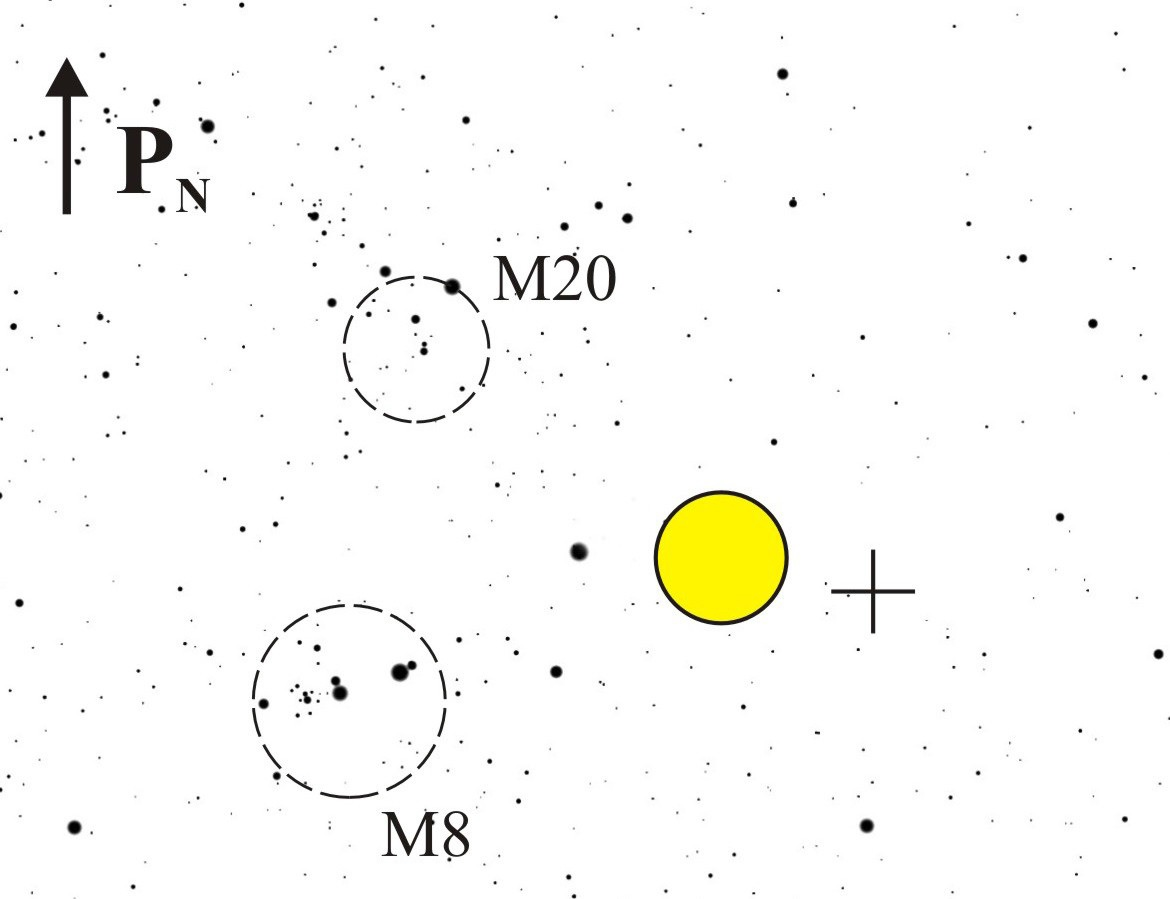
\includegraphics[scale=0.25]{sol-merc.jpg}}
    \end{figure}
    \item Предположим, Вы стали свидетелем редчайшего явления для Земли: Марс, находясь в точке западной квадратуры, прошел по диаметру диска Юпитера. Сколько времени будет длиться это явление (вместе с частными фазами) в одном пункте нашей планеты? Эксцентриситетом и наклоном орбит планет к плоскости эклиптики, движением наблюдателя за счет осевого вращения Земли пренебречь.
    \item Эксцентриситет орбиты искуственного спутника Земли $0.8$. Сравните его угловые скорости в апогее и перигее для условного наблюдателя, находящегося в центре Земли.
    \item Угловая скорость планеты в фокальном параметре и в апоцентре различается в $4$ раза при наблюдении с центральной звезды. Найдите эксцентриситет орбиты.
    \item Некоторый спутник обращается вокруг Земли по орбите с высотой $h = 300$~км в плоскости земного экватора. Найдите промежуток времени, в течение которого он будет над горизонтом для наблюдателя на экваторе за один оборот вокруг Земли. Угловой скоростью Земли по сравнению с угловой скоростью спутника пренебречь.
    \item Определите угловой размер Марса в западной квадратуре, а также его лучевую скорость. Орбиты Марса и Земли считать круговыми и лежащим в одной плоскости. 
    \item Марс находится в западной квадратуре. Ответьте на следующие вопросы: 
    \begin{enumerate}
        \item Чему будет равно отношение лучевой и полной пространственной скорости планеты относительно земного наблюдателя?
        \item Чему будет равно отношение лучевой и полной скорости планеты в случаях противостояния и соединения?
    \end{enumerate}
    \item Определите максимальную лучевую скорость астероида, двигающегося по круговой орбите с синодическим периодом $0.3$ года.
    \item В момент наибольшей восточной квадратуры для земного наблюдателя лучевая скорость астероида составила $+20$ км/с. Определите радиус орбиты астероида, считая её круговой и лежащей в плоскости эклиптики. Направления вращения Земли и астероида совпадают.
    \item Смещение линии $H_{\gamma}$ ($4341$~\AA) составляет $5$~\AA. Определите скорость движения источника.
\end{enumerate}
\end{document}